% Тут используется класс, установленный на сервере Papeeria. На случай, если
% текст понадобится редактировать где-то в другом месте, рядом лежит файл matmex-diploma-custom.cls
% который в момент своего создания был идентичен классу, установленному на сервере.
% Для того, чтобы им воспользоваться, замените matmex-diploma на matmex-diploma-custom
% Если вы работаете исключительно в Papeeria то мы настоятельно рекомендуем пользоваться
% классом matmex-diploma, поскольку он будет автоматически обновляться по мере внесения корректив
%

% По умолчанию используется шрифт 14 размера. Если нужен 12-й шрифт, уберите опцию [14pt]
%\documentclass[14pt]{matmex-diploma}
\documentclass[14pt]{matmex-diploma-custom}
\usepackage{fontspec}
\usepackage{polyglossia}
\usepackage{amsmath}
\usepackage{amsfonts}
\usepackage{amssymb}

% пакеты из презентации
\usepackage{algpseudocode}
\usepackage{algorithm}
\usepackage{algorithmicx}
\usepackage{pdfpages}


\usepackage{geometry}
\usepackage{amsfonts,latexsym}
\usepackage{amsthm}
\usepackage{amssymb}
\usepackage[utf8]{inputenc} % Кодировка
\usepackage{mathtools}
\usepackage{hyperref}
\usepackage{tikz}
\usepackage{dsfont}
\usepackage{multicol}
\usetikzlibrary{fit,calc,automata,positioning}

\usepackage{fontawesome}

\theoremstyle{definition}
\newtheorem{definition}{Определение}[section]
\newtheorem{example}{Пример}[section]
\newtheorem{theorem}{Теорема}[section]
\newtheorem{proposition}[theorem]{Proposition}
\newtheorem{lemma}[theorem]{Лемма}
\newtheorem{corollary}[theorem]{Corollary}
\newtheorem{conjecture}[theorem]{Conjecture}
\newtheorem{note}[theorem]{Утверждение}

\begin{document}
% Год, город, название университета и факультета предопределены,
% но можно и поменять.
% Если англоязычная титульная страница не нужна, то ее можно просто удалить.
\filltitle{ru}{
    chair              = {Программная инженерия},
    title              = {Модернизация набора данных \textsc{CFPQ\_Data}},
    % Здесь указывается тип работы. Возможные значения:
    %   coursework - Курсовая работа
    %   diploma - Диплом специалиста
    %   master - Диплом магистра
    %   bachelor - Диплом бакалавра
    type               = {coursework},
    position           = {студента},
    group              = 371,
    author             = {Абзалов Вадим Игоревич},
    supervisorPosition = {к.\,ф.-м.\,н., доцент кафедры информатики СПбГУ},
    supervisor         = {С.\,В. Григорьев},
%   university         = {Санкт-Петербургский Государственный Университет},
%   faculty            = {Математико-механический факультет},
%   city               = {Санкт-Петербург},
%   year               = {2019}
}

\maketitle
\tableofcontents

\section{Introduction}


Language-constrained path querying~\cite{barrett2000formal} is a technique for graph navigation querying.
This technique allows one to use formal languages as constraints on paths in edge-labeled graphs: path satisfies constraints if labels along it form a word from the specified language.

The utilization of regular languages as constraints, or \textit{Regular Path Querying} (RPQ), is most well-studied and widespread.
Different aspects of RPQs are actively studied in graph databases~\cite{10.1145/2463664.2465216, 10.1145/3104031,10.1145/2850413}, while regular constraints are supported in such popular query languages as PGQL~\cite{10.1145/2960414.2960421} and SPARQL\footnote{Specification of regular constraints in SPARQL property paths: \url{https://www.w3.org/TR/sparql11-property-paths/}. Access date: 07.07.2020.}~\cite{10.1007/978-3-319-25007-6_1} (property paths).
Nevertheless, there is certainly room for improvement of RPQ efficiency, and new solutions are being created~\cite{Wang2019,10.1145/2949689.2949711}.

At the same time, using more powerful languages, namely context-free languages, as constraints has gained popularity in the last few years.
\textit{Context-Free Path Querying} problem (CFPQ) was introduced by Mihalis Yannakakis in 1990 in~\cite{Yannakakis}.
Many algorithms were proposed since that time, but recently, Jochem Kuijpers et al. showed in~\cite{Kuijpers:2019:ESC:3335783.3335791} that state-of-the-art CFPQ algorithms are not performant enough for practical use.
This motivates us to develop new algorithms for CFPQ.

One promising way to achieve high-performance solutions for graph analysis problems is to reduce them to linear algebra operations.
This way, GraphBLAS~\cite{7761646} API, the description of basic linear algebra primitives, was proposed.
Solutions that use libraries that implement this API, such as SuiteSparce~\cite{10.1145/3322125} and CombBLAS~\cite{10.1177/1094342011403516}, show that reduction to linear algebra is a way to utilize high-performance parallel and distributed computations for graph analysis.

Rustam Azimov shows in~\cite{Azimov:2018:CPQ:3210259.3210264} how to reduce CFPQ to matrix multiplication.
Later, it was shown in~\cite{Mishin:2019:ECP:3327964.3328503} and~\cite{10.1145/3398682.3399163} that utilization of appropriate libraries for linear algebra for Azimov's algorithm implementation makes a practical solution for CFPQ.
However Azimov's algorithm requires transforming the input grammar to Chomsky Normal Form, which leads to the grammar size increase, and hence worsens performance, especially for regular queries and complex context-free queries.

To solve these problems, an algorithm based on automata intersection was proposed~\cite{10.1007/978-3-030-54832-2_6}.
This algorithm is based on linear algebra and does not require the transformation of the input grammar.
We improve the algorithm in this work.
We reduce the above mentioned solution to operations over Boolean matrices, thus simplifying its description and implementation.
Also, we show that this algorithm is performant enough for regular queries, so it is a good candidate for integration with real-world query languages: one algorithm can be used to evaluate both regular and context-free queries.

Moreover, we show that this algorithm opens the way to tackle a long-standing problem about the existence of truly-subcubic $O(n^{3-\epsilon})$ CFPQ algorithm ~\cite{10.1145/1328438.1328460, Yannakakis}.
Currently, the best result is an $O(n^3/\log{n})$ algorithm of Swarat Chaudhuri~\cite{10.1145/1328438.1328460}.
Also, there exist truly subcubic solutions which use fast matrix multiplication for some fixed subclasses of context-free languages~\cite{8249039}.
Unfortunately, this solutions cannot be generalized to arbitrary CFPQs.
In this work, we identify incremental transitive closure as a bottleneck on the way to achieve subcubic time complexity for CFPQ.

To sum up, we make the following contributions.
\begin{enumerate}
	\item We rethink and improve the CFPQ algorithm based on tensor-product proposed by Orachev et al. ~\cite{10.1007/978-3-030-54832-2_6}.
	We reduce this algorithm to operations over Boolean matrices.
	As a result, all-path query semantics is handled, as opposed to the previous matrix-based solution which handles only the single-path semantics.
	Also, both regular and context-free grammars can be used as queries.
	We prove the correctness and time complexity for the proposed algorithm.
	\item We demonstrate the interconnection between CFPQ and incremental transitive closure.
	We show that incremental transitive closure is a bottleneck on the way to achieve faster CFPQ algorithm for general case of arbitrary graphs as well as for special families of graphs, such as planar graphs.
	\item We implement the described algorithm and evaluate it on real-world data for both RPQ and CFPQ. Results show that the proposed solution is comparable with existing solutions for CFPQ and RPQ, thus it is a promising way to create a unified algorithm for both CFPQ and RPQ evaluation.
\end{enumerate}
% Обязательный слайд: четкая формулировка цели данной работы и постановка задачи
% Описание выносимых на защиту результатов, процесса или особенностей их достижения и т.д.
\begin{frame}
	\transwipe[direction=90]
	\frametitle{\faThumbTack\ Цель и задачи}
	\textbf{Цель}: модернизация существующего набора данных \textsc{CFPQ\_Data} для создания унифицированного средства подготовки проведения экспериментального исследования CFPQ алгоритмов
	  
	~\
	  
	\textbf{Задачи}
	
	\newline
	
	\begin{itemize}
		\item[\bullet] Модернизация архитектуры набора данных
		\item[\bullet] Добавление новых возможностей работы с данными
		      \begin{itemize}
		      	\item[\bullet] Загрузка конкретных графов из набора данных
		      	\item[\bullet] Преобразование графов в другие форматы
		      	\item[\bullet] Получение информации о графе
		      	\item[\bullet] Трансформация графов
		      \end{itemize}
% 		\item[\bullet] Разработка и реализация протокола версионирования данных
		\item[\bullet] Публикация Python пакета для работы с набором данных и документации к нему
	\end{itemize}
	
\end{frame}


\section{Обзор}

Прежде чем приступать к модернизации \textsc{CFPQ\_Data} необходимо разобраться, какие стандарты оформления наборов данных приняты в современном мире.

\subsection{Наборы графовых данных}

Стоит отметить, что существует множество различных наборов графовых данных~\cite{BoVWFI, BRSLLP, SNAPDATESETS}.
Так, например, проект <<SNAP: Stanford Network Analysis Project>>~\cite{SNAPDATESETS}, который начал активно развиваться в 2004 году в результате исследований по анализу крупных социальных и информационных сетей.
Крупнейшей сетью, которая была проанализирована с помощью библиотеки, была сеть <<Micro\-soft Instant Messenger>> 2006 года, содержащая 240 миллионов вершин и 1,3 миллиарда ребер.
Наборы данных~\cite{SNAPDATESETS}, доступные на веб-сайте библиотеки WebGraph\footnote{Веб-сайт библиотеки <<SNAP: Stanford Network Analysis Project>>: \url{https://snap.stanford.edu/}, дата последнего доступа --- 04.06.2021}, были собраны для целей этих исследований.
Сам набор данных оформлен в виде нескольких таблиц, отвечающих различным прикладным областям, из которых были извлечены графы.
При этом каждая таблица содержит: ссылку на страницу с описанием графа, тип абстракции графа (ориентированный / неориентированный, с весами / без весов и т.п.), количество вершин, количество рёбер и описание того, откуда был извлечён граф.

В работах <<The webgraph framework I: compression techniques>>~\cite{BoVWFI} и <<Layered Label Propagation: A MultiResolution Coordinate-Free Ordering for Compressing Social Networks>>~\cite{BRSLLP} предлагаются новые методы сжатия графов социальных и информационных сетей.
Это важно, поскольку изучение таких графов часто затруднено из-за их большого размера.
На основе этих работ был разработан фреймворк <<WebGraph>> --- набор алгоритмов и инструментов, направленных на упрощение манипулирования большими графами.
С помощью это фреймворка были получены компактные представления различных графов реальных социальных и информационных сетей.
Все эти наборы данных представлены на веб-сайте проекта\footnote{Веб-сайт проекта <<WebGraph>>: \url{http://law.di.unimi.it/datasets.php}, дата последнего доступа --- 04.06.2021}.
Они также оформлены в виде нескольких таблиц.
Каждая таблица содержит: ссылку на страницу с описанием графа, дату загрузки графа, количество вершин и рёбер.

Все эти проекты, собирающие наборы данных для исследований в своих прикладных областях, так или иначе выделяют некоторую общую информацию о каждом графе: описание графа, количество вершин и рёбер.
Подобные данные обязательно должны быть включены в \textsc{CFPQ\_Data}.

Для CFPQ алгоритмов ключевую роль играют метки на рёбрах, которые представляют различные отношения между вершинами графа.
Именно поэтому, указанные выше наборы данных, не подходят для подготовки экспериментального исследования CFPQ алгоритмов, поскольку представляют собой наборы непомеченных графов.
Попытки же синтетического добавления меток могут привести к полной потере всей практической ценности этих графов.

\subsubsection{Наборы графовых данных для задачи с регулярными ограничениями}

Существует довольно много различных наборов данных для экспериментального исследования алгоритмов, реализующих регулярные запросы \cite{RBench, GSCALER, gMark}.
Например, проект <<RBench>>~\cite{RBench} для создания масштабируемых синтетических наборов графовых данных по данному набору графов, представленных в формате RDF.
Однако регулярные запросы представляют более узкий класс, чем контекстно-свободные, что не позволяет в полной мере использовать такие данные для экспериментального исследования CFPQ алгоритмов.

Формат RDF был выбран в качестве основной модели представления графов консорциумом <<W3C>>~\cite{SEMANTICWEB} и, благодаря этому, имеет широкую поддержку.
Он позволяет описывать отношения между ресурсами в виде <<объект, предикат, субъект>>, что идеально соответствует абстракции помеченного графа.
Именно по этим причинам данный формат был выбран в качестве стандартного представления графов, собранных в \textsc{CFPQ\_Data}.

\subsubsection{Наборы графовых данных для задачи с кон\-текст\-но-свобод\-ны\-ми ограничениями}

Графы и грамматики, представляющие наборы данных для подготовки экспериментального исследования CFPQ алгоритмов представлены весьма разрозненно, что вызвано отсутствием единого набора данных и проблемой создания помеченных графов исключительно под соответствующие экспериментальные нужды.

Например, набор популярных онтологий, связанных с концепцией семантической паутины~\cite{SEMANTICWEB}, который можно найти в работе <<Context-Free Path Queries on RDF Graphs>>~\cite{CFPQORDFG}.
Графы именно оттуда наиболее часто использовались для подготовки экспериментального исследования CFPQ алгоритмов.
К сожалению, они достаточно небольшие (несколько сотен вершин), что не позволяет использовать их для исследования практической применимости CFPQ алгоритмов.
Однако, для простой проверки того, что CFPQ алгоритм работает, такие данных отлично подходят. 

Недавно появилась работа <<An Experimental Study of Context-Free Path Query Evaluation Methods>>~\cite{ANESOFCFPQEM}, в которой представлены графы гораздо большего размера (от нескольких тысяч до первых миллионов вершин), что уже позволяет использовать их для исследования практической применимости CFPQ алгоритмов.
Поскольку такие графы по своим размерам гораздо лучше соответствуют тем помеченным графам, которые извлекались из различных практических областей в других наборах графовых данных~\cite{BoVWFI, BRSLLP, SNAPDATESETS}.

 В работах <<Batch alias analysis>>~\cite{BAA} и <<Demand-driven alias analysis for C>>~\cite{DDAAFORC} используются помеченные графы, представляющие данные для задачи поиска объектов ссылающихся на одни и те же места в памяти.
 Так как эта задача сводится к поиску путей с кон\-текст\-но-свобод\-ными ограничениями, то граф, построенный для её решения, однозначно соответствует абстракции помеченного графа, используемой в CFPQ алгоритмах.

Графы из представленных выше работ~\cite{CFPQORDFG, ANESOFCFPQEM, BAA, DDAAFORC} уже добавлены в \textsc{CFPQ\_Data}.
Поскольку они идеально соответствуют абстракции помеченного графа и представляют реальные данные из различных прикладных областей, что позволяет полноценно использовать их для подготовки экспериментального исследования CFPQ алгоритмов.

В работе <<Subgraph Queries by Context-free Grammars>>~\cite{SQBYCFG} для экспериментального исследования нового CFPQ алгоритма синтезирован граф на примерно 1 миллион вершин и примерно 5.7 миллионов рёбер путём объединения набора общедоступных источников данных: UniProt (белки), Entrez Gene (гены), Gene Ontology (функции белков, биологические процессы и клеточные местоположения), InterPro (семейства белков и консервативные домены), KEGG (биохимические пути), OMIM (отношения ген-фенотип), HomoloGene (группы гомологии генов) и STRING (взаимодействия белков).
Подобный подход к подготовке экспериментального исследования с одной стороны, является весьма перспективным, поскольку позволяет синтезировать помеченные графы любых размеров, отвечающие реальным данным, но, с другой стороны, требует весьма глубокого понимания структуры самих данных, которые будут использованы для построения графа.
Именно поэтому данный способ не применяется в \textsc{CFPQ\_Data}.

\subsection{Проект \textsc{CFPQ\_Data}}

Из-за проблемы разрозненности наборов графовых данных, подходящих для использования в экспериментальном исследовании CFPQ алгоритмов, графы из работ <<Context-Free Path Queries on RDF Graphs>>~\cite{CFPQORDFG}, <<An Experimental Study of Context-Free Path Query Evaluation Methods>>~\cite{ANESOFCFPQEM}, <<Batch alias analysis>>~\cite{BAA} и <<Demand-driven alias analysis for C>>~\cite{DDAAFORC} были собраны в единый набор данных, который получил название \textsc{CFPQ\_Data}.

Также в него были добавлены функции для генерации синтетических графов для особых случаев: теоретически доказанный худший случай запроса в виде языка правильных скобочных последовательностей на графе, состоящем из двух циклов~\cite{QFORPINGUCFPQ}; разреженные графы для симуляции реальных данных; графы, результат вычисления запроса на которых является теоретически максимальным; случайные безмасштабные сети, для генерации которых применяется модель Барабаши-Альберта~\cite{SMOFCN}.
А также функции для преобразования кон\-текстно-свобод\-ной грамматики выбранного формата в нормальную форму Хомского.

Но проект \textsc{CFPQ\_Data} имеет ряд технических проблем, не позволяющих в полной мере насладиться процессом подготовки экспериментального исследования CFPQ алгоритмов.
Так, вместо того, чтобы предоставить исследователям возможность загружать конкретный граф, набор данных загружается целиком, что становится критической проблемой при увеличении количества графов в наборе.
При этом в самом наборе данных имеется информация лишь о названиях графов в нем содержащихся, что не соответствует принятым в сообществе стандартам оформления наборов графовых данных.
Кроме того, все функции, предоставляемые проектом \textsc{CFPQ\_Data}, доступны пользователю через единственный интерфейс командной строки, что крайне, крайне радикально ограничивает возможности по взаимодействию с набором данных и подготовке экспериментального исследования замечательных CFPQ алгоритмов.

\section{Модернизация набора данных \textsc{CFPQ\_Data}}

В результате обзора предметной области в проект \textsc{CFPQ\_Data} были внесены следующие изменения.
\begin{itemize}
    \item Было изменено стандартное представление графов и грамматик.
    \item Обновлено и расширено множество функций, предоставляемых проектом.
    \item Доступ к набору данных изменен с интерфейса командной строки на Python пакет, опубликованный в PYPI\footnote{Python пакет <<\textsc{CFPQ\_Data}>>: \url{https://pypi.org/project/cfpq-data/}, дата последнего доступа --- 04.06.2021}.
    \item Добавлено и автоматизировано интеграционное тестирование.
    \item Обновлен веб-сайт и автоматизирована его публикация.
\end{itemize}

\subsection{Представление данных}

Представление графа в виде множества записей вида <<объект, предикат, субъект>> хотя и идеально соответствует структуре помеченного графа и позволяет компактным образом хранить граф, но не подходит для исследования и манипулирования графами.
Именно поэтому в качестве стандартного представления помеченного графа выбран класс <<MultiDiGraph>> из проекта <<networkx>>\footnote{GitHub репозиторий <<networkx>>: \url{https://github.com/networkx/networkx}, дата последнего доступа --- 04.06.2021}, который является одним из наиболее известных проектов для работы с графами, хорошо задокументирован и имеет внушительное сообщество.
Такое архитектурное решение позволяет применять к графам, имеющимся в \textsc{CFPQ\_Data}, весь богатый арсенал функций из проекта <<networkx>>, что несомненно упрощает их исследование и манипулирование ими.

По тем же причинам, в качестве стандартного представления кон\-текстно-свобод\-ной грамматики выбран класс <<CFG>> из проекта <<py\-form\-lang>>\footnote{GitHub репозиторий <<py\-form\-lang>>: \url{https://github.com/Aunsiels/pyformlang}, дата последнего доступа --- 04.06.2021}, который является одним из наиболее известных проектов для работы с формальными языками и, в том числе, с контекстно-свободными грамматиками.
Кроме того, было реализовано представление контекстно-свободной грамматики с помощью рекурсивного автомата~\cite{RSM}.

\subsection{Архитектура}

Все предоставляемые для работы с графами и грамматиками функции выделены в один пакет <<\textsc{CFPQ\_Data}>>.

\begin{figure}[h]
    \centering
    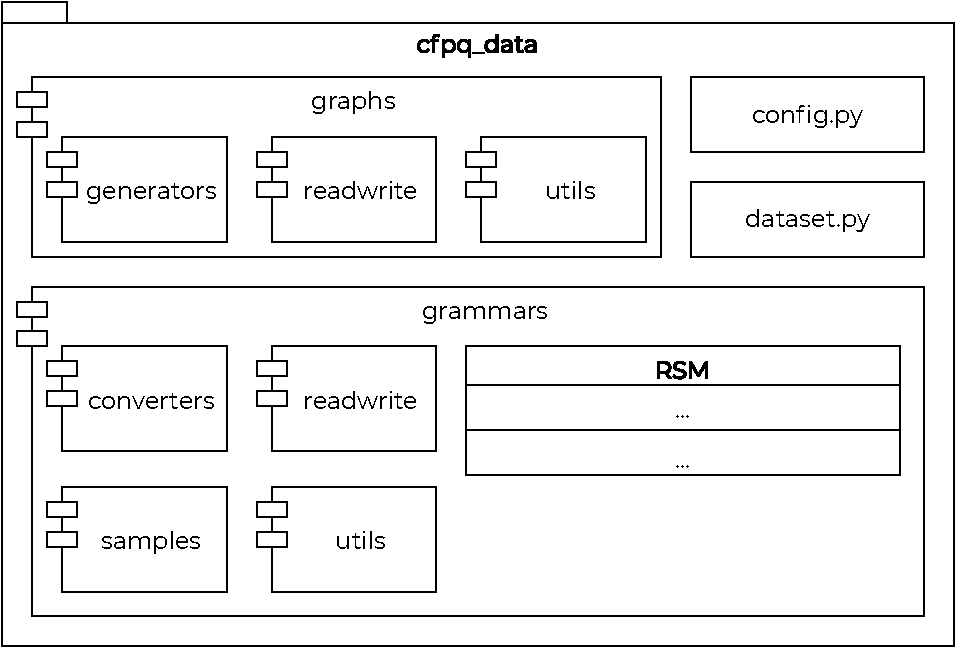
\includegraphics[width=\textwidth]{img/architecture_new.pdf}
    \caption{Новая архитектура \textsc{CFPQ\_Data}}
\end{figure}

Функции для манипулирования графами собраны в модуле <<graphs>>, который состоит из трех подмодулей.
\begin{itemize}
    \item В подмодуле <<generators>> реализованы функции генерации синтетических графов.
    \item В подмодуле <<readwrite>> реализованы функции чтения и записи графов, представленных в формате RDF и в формате троек <<вершина, метка ребра, вершина>>.
    \item В подмодуле <<utils>> реализованы функции для трансформации графов.
\end{itemize}

Функции для манипулирования грамматиками собраны в модуле <<grammars>>, который состоит из четырех подмодулей.
\begin{itemize}
    \item В подмодуле <<converters>> реализованы функции конвертации кон\-текстно-свобод\-ной грамматики между различными представлениями.
    \item В подмодуле <<readwrite>> реализованы функции чтения и записи кон\-текстно-свобод\-ной грамматики, представленной в различных форматах.
    \item В подмодуле <<samples>> реализованы примеры кон\-текстно-свобод\-ных запросов для соответствующих помеченных графов из <<graphs>>.
    \item В подмодуле <<utils>> реализованы функции для трансформации грамматик.
\end{itemize}

В файле <<dataset.py>> фиксируется информация о графах, сохраненных в \textsc{CFPQ\_Data}, соответствующая версии пакета, а в файле <<config.py>> фиксируется конфигурация доступа пакета к набору данных.

Также, с помощью GitHub Actions\footnote{GitHub Action интеграционного тестирования: \url{https://github.com/JetBrains-Research/CFPQ_Data/actions/workflows/tests.yml}, дата последнего доступа --- 04.06.2021} было реализовано интеграционное тестирование полученного пакета на юнит-тестах на различных операционных системах, с последующим сбором информации о покрытии кода.

\subsection{Документация}
Все предоставляемые пользователю функции были снабжены документацией, публикация которой добавлена в новой версии веб-сайта проекта.
Также на веб-сайт были добавлены следующие страницы.
\begin{itemize}
    \item Страница\footnote{<<Dataset>>: \url{https://jetbrains-research.github.io/CFPQ_Data/dataset/index.html}, дата последнего доступа --- 04.06.2021} с описанием графов из набора данных \textsc{CFPQ\_Data}.
    \item Страница\footnote{<<Install>>: \url{https://jetbrains-research.github.io/CFPQ_Data/install.html}, дата последнего доступа --- 04.06.2021} с руководством по установке пакета.
    \item Страница\footnote{<<Tutorial>>: \url{https://jetbrains-research.github.io/CFPQ_Data/tutorial.html}, дата последнего доступа --- 04.06.2021} с руководством помогающим начать пользоваться пакетом.
    \item Страница\footnote{<<Reference>>: \url{https://jetbrains-research.github.io/CFPQ_Data/reference/index.html}, дата последнего доступа --- 04.06.2021} с документацией всех функций, имеющихся в пакете.
    \item Страница\footnote{<<About>>: \url{https://jetbrains-research.github.io/CFPQ_Data/about.html}, дата последнего доступа --- 04.06.2021} с информацией о группе разработчиков проекта.
    \item Страница\footnote{<<License>>: \url{https://jetbrains-research.github.io/CFPQ_Data/license.html}, дата последнего доступа --- 04.06.2021} с лицензией проекта.
\end{itemize}

Также было сохранено индексирование проекта в Google Dataset Search и автоматизирована публикация сайта на GitHub Pages с помощью GitHub Actions\footnote{GitHub Action публикации веб-сайта: \url{https://github.com/JetBrains-Research/CFPQ_Data/actions/workflows/deploy_docs.yml}, дата последнего доступа --- 04.06.2021}.
\section{Conclusion}

Conclusion, current state, results.

Future work. Library extension up to full GraphBLAS API implementation.

LaGraph on F\# .NET.

Evaluation. Comparison with other implementations on different devices.
Manual implementation versus translation.  

Another direction of future work is Brahma.FSharp improvements. 
First of all, it is necessary to support discriminated unions to make it possible to express custom semirings such as \texttt{Min-Plus}, as presented in listing~\ref{lst_example}. 

Also, it is necessary to add high-level abstractions for asynchronous programming, and for multi-GPU programming.
Such mechanisms can be naturally expressed in F\# with native primitives for asynchronous programming.

fusion and other optimizations.

\setmonofont[Mapping=tex-text]{CMU Typewriter Text}
\bibliographystyle{ugost2008ls}
\bibliography{diploma.bib}
\end{document}